%$Id$
\documentclass[a4paper,12pt]{article}
\usepackage[utf8]{inputenc}
%\usepackage[spanish]{babel}
\usepackage{pslatex} %Para el pdf sea más mono.
\usepackage{eurosym}
\usepackage{amssymb}
\usepackage{latexsym}
\usepackage[dvips]{graphicx}
\usepackage{delarray}
\usepackage{amsmath}
%\usepackage{bbm}
%\usepackage{bbold}
%\usepackage{accents}
\usepackage{subfigure}
\usepackage{multirow}
\usepackage{fancyhdr}
%\usepackage{tocbibind} % Para que incluya la bibliografia en el indice
%\usepackage{bibtex}
\usepackage{wrapfig}
\usepackage{color}
\usepackage{hyperref}
%\usepackage{fmtcount}
\usepackage{parskip}
\frenchspacing

\graphicspath{{./fig/}{./png/}}

\setlength{\hoffset}{-1in}
\setlength{\textwidth}{7.5in}
\setlength{\voffset}{-1.2in}
\setlength{\textheight}{10.0in}

\title{Pencil-code: quick reference guide.}

\author{Illa R. Losada, Michiel Lambrechts, Elizabeth Cole }


\begin{document}
\maketitle

\tableofcontents

\newpage

\section{Download the Pencil Code}
The Pencil Code is an open source code. General information can be found at

\url{http://www.nordita.org/pencil-code/}.


You need \verb|svn| to download the latest version 
\begin{verbatim}
svn checkout https://pencil-code.googlecode.com/svn/trunk/ pencil-code
--username NAME
\end{verbatim}

where you replace NAME by your gmail name, and the password is the
one generated by pencil-code.googlecode.com ($\rightarrow$profile
$\rightarrow$settings). 

An alternative for a non-up-to-date version of the pencil-code is
\url{
wget http://pencil-code.googlecode.com/files/pencil-code-r18525.tar.gz
}

The downloaded \verb|pencil-code| directory contains several sub-directories
\begin{enumerate}
  \item \verb|samples|:  many sample problems
  \item \verb|config|: all the configuration files.
  \item \verb|doc| a very important directory containing the pencil-code
    \verb|manual.tex|
  \item \dots
\end{enumerate}
For example, the code structure can be further explored in Section 4 of the
manual.

\section{Configure the shell}

<<<<<<< .mine
I the \verb|tcsh| shell, put in your \$HOME/.cshrc file the following lines:
=======
It is recommend to use cshell instead of bash.

Under the tcsh shell, put in your \$HOME/.cshrc file the following lines:
>>>>>>> .r19030
\begin{verbatim}
#
#  path for pencil code
#
if (! $?PENCIL_HOME) setenv PENCIL_HOME $HOME/pencil-code
if (-r $PENCIL_HOME/sourceme.csh) then
  set _sourceme_quiet; source $PENCIL_HOME/sourceme.csh; unset _sourceme_quiet
endif
\end{verbatim}

Note: If you want to change your default \$SHELL to tcsh, type

\begin{verbatim}
  chsh
  /bin/tcsh
\end{verbatim}

The first command prompts you for your normal unix password.

If you are under the bash shell, put in your \$HOME/.bashrc file the following
lines:
\begin{verbatim}
#
#  path for pencil code
#
if [ -z $PENCIL_HOME ]; then  export PENCIL_HOME=$HOME/pencil-code; fi
if [ -e $PENCIL_HOME/sourceme.sh ]; then
  set _sourceme_quiet; source $PENCIL_HOME/sourceme.sh; unset _sourceme_quiet
fi
\end{verbatim}

Also add the following useful alias:

With tcsh: \texttt{alias pc 'cd \$PENCIL\_HOME'}
With bash: \texttt{alias pc='cd \$PENCIL\_HOME'}

such that you will directly move to the Pencil Code directory wherever you are
by typing 'pc'.

Source your updated \$HOME/.cshrc or \$HOME/.bashrc file by typing:

With tcsh: \texttt{source .cshrc}
With bash: \texttt{source .bashrc}

\section{Configure makefile.}

In order to run the code a proper configuration file is needed. This file should contain all the information related with the compilers and their special options.

The configuration files should be located in the \verb|config| directory and should have a special name related with the host-id. This id is easyly obtained by:  
\begin{verbatim}
pc_build --debug
\end{verbatim}
And now create a new config file in:
\texttt{config/hosts/YOUR-NAME/HOST-ID.conf}

The next step is customize this file, there are several examples in \verb|$PENCIL_HOME/config/hosts|. 


\section{Useful commands.}
\begin{center}
\begin{tabular}{|l|l|}\hline
pc & move to the PC directory\\\hline
cd samples/conv-slab & move to the sample 'conv-slab' which is in a 'samples'
directory\\\hline
pc\_setupsrc & initialize the local 'src' directory, copy necessary files,
etc...\\\hline
make & 	compile the code\\\hline
mkdir data & create the data directory where all the outputs will be written
\\\hline
start.csh & compute the initial setup at time t=0 \\\hline
run.csh & launch the main code that advances the equations in time\\\hline
\end{tabular}
\end{center}

\section{Configure the run}
The structure of the Pencil code consists of different modules, containing
different physics that you may or may not need for your problem. 

\subsection{Makefile}

\begin{verbatim}
pc_setupsrc
\end{verbatim}
This sets up the linking to the root \verb|src| directory and makes a
\verb|data| directory that will contain the data produced by your simulation.

Basic configuration files for the make:
\begin{verbatim}
src/Makefile.local
src/cparam.local
\end{verbatim}

The structure of the Pencil code consists of different modules, containing
different physics that you may or may not need for your problem. These are set
in \verb|Makefile.local|. 

Example of a file without mpi:
\begin{verbatim}
###                             -*-Makefile-*-
### Makefile for modular pencil code -- local part
### Included by `Makefile'
###

MPICOMM=nompicomm
#MPICOMM=mpicomm
GRAVITY=gravity_simple
EOS=eos_idealgas
FORCING=noforcing
ENTROPY=noentropy
MAGNETIC=magnetic
MAGNETIC_MEANFIELD=magnetic/meanfield
DENSITY=density
HYDRO=hydro
\end{verbatim}

The \texttt{src/cparam.local} file set the local settings concerning grid size
and number of CPUs. My file (no mpi):
\begin{verbatim}
!  -*-f90-*-  (for Emacs)    vim:set filetype=fortran:  (for vim)
!
!  cparam.local
!
!  Local settings concerning grid size and number of CPUs.
!  This file is included by cparam.f90
!
integer, parameter :: ncpus=1,nprocx=1,nprocy=1,nprocz=ncpus/(nprocx*nprocy)
integer, parameter :: nxgrid=128,nygrid=1,nzgrid=128
!
\end{verbatim}

\subsection{Run configuration files}

There are three basic configuration files where all the physics and outputs are specify: print.in, run.in and start.in.
\begin{itemize}
 \item \verb|print.in|: write here all the input magnitudes you need.
  \item \verb|run.in|: parameters values, number of timesteps,...
  \item \verb|start.in|: Initialisation parameters
\end{itemize}



%\section{Running the code}
%
%In order to use the code, a compilation in each of the working directories is
%needed. Basically there are two ways of compiling and running the code.
%The only way of using the Makefile config file created before is using the new
%way:
%
%The standard way:
%\begin{enumerate}
%  \item \verb|pc_build| compile the code
%  \item \verb|pc_run| run the code
%    \begin{enumerate}
%      \item \verb|pc_run start| can be run before \verb|pc_run|, to construct
%        the initial condition.
%    \end{enumerate}
%\end{enumerate}

%The old way of doing it was:
%\begin{verbatim}
%make
%./start.csh
%./run.csh
%\end{verbatim}
%But one usually need to specify some options by hand in the make command. In my
%case, to use mpi:
%\begin{verbatim}
%make FC=mpif90
%\end{verbatim}
    
\section{Setting up python.}
\subsection{Python modules requirements.}
The basic needed modules are: numpy and matplotlib.
\begin{itemize}
 \item numpy: all array definitions and operations.
  \item matplotlib: plotting.
\end{itemize}

Other really useful modules are: ipython and scipy.

\begin{itemize}
 \item ipython: enhanced python interpreter.
  \item scipy: science functions and utilities.
\end{itemize}


\subsection{Installation}
Untar the \texttt{tar.gz} file or go to the directory and simple type as root or sudoed:
\begin{verbatim}
python setup.py install
\end{verbatim}
For a user installation (no root permision):
\begin{verbatim}
python setup.py install --user
\end{verbatim}

\subsection{Using the module.}
Import the module:
\begin{verbatim}
import pencil as pc
\end{verbatim}
Some useful functions:
\begin{center}
\begin{tabular}{|l|l|}\hline
pc.read\_ts & Read ``time\_series.dat'' file. Parameters are added as members of the class. \\\hline
pc.read\_slices & read 2D slice binary files and return two arrays: one of (nslices,vsize,hsize) and other of time\\\hline
pc.animate\_interactive &  Assemble a 2D animation from a 3D array. \\\hline
%× & ×\\\hline
%× & ×\\\hline
%× & ×\\\hline
\end{tabular}
\end{center}

\section{Run a sample: an example}
% TODO Searching in the pencil code
% 1D Jeans sample?
% Please feel free to change this sample if it is not to your liking. 

Construct a folder in which you would like to run the sample
\begin{verbatim}
 > mkdir sample_test_jeans
\end{verbatim}

Now we copy the sample from the pencil code directory
\begin{verbatim}
 > pc_newrun ~/pencil-code/samples/1d-tests/jeans-x jeans-x
\end{verbatim}

The \verb|pc_setupsrc| command sets up the linking to the root \verb|src|
directory and makes a
\verb|data| directory that will contain the data produced by your simulation.
\begin{verbatim}
 /jeans-x> pc_setupsrc
\end{verbatim}

You can inspect the included modules in
\begin{verbatim}
 /jeans-x> vi src/Makefile.local 
\end{verbatim}
where I used the \verb|vi| text editor. The grid size can be inspected in 
\begin{verbatim}
 /jeans-x> vi src/cparam.local 
\end{verbatim}

The code is compiled by
\begin{verbatim}
 /jeans-x> pc_build
\end{verbatim}
and this may take some time.

The initial conditions are set in
\begin{verbatim}
 /jeans-x> vi start.in
\end{verbatim}

and parameters necessary to run the code in time can be found in
\begin{verbatim}
 /jeans-x> vi run.in
\end{verbatim}

Time to run the code. 
\begin{verbatim}
 /jeans-x> pc_run
\end{verbatim}

Visualizing the output can be either done with \verb|idl| or \verb|python|.

\subsection{IDL visualisation}
% The goal of this section is to demonstrate the general workflow with a very
% simple example.

Start \verb|idl| from the command line. Several \verb|idl| have been written (you can find them in
\verb|pencil-code/idl| ) to facilitate inspecting the data (which can be found
in raw format in \verb|jeans-x/data| directory).  For example, let us inspect
the time series data.
\begin{verbatim}
IDL> pc_read_ts, obj=ts
\end{verbatim}

\section{Another example: helically forced turbulence.}


%\section{Question 1}
\textbf{Simulate the saturation behaviour of a dynamo from helically forced turbulence with forcing wave-number $k_f = 3$ in units of the box wave-number $k_1 = 1$.}

During  this question I will use the example configuration \texttt{samples/helical-MHDturb}, changing different parameters though the questions.

\subsection{Critical value for the magnetic diffusivity.}

Calculation of the critical value for the magnetic diffusivity implies running the code for different values of the magnetic diffusivity and checking up at which value the field starts growing.

Since the proposed value for $\eta$ ($\eta = 2e-3$) corresponds to a growing field, I have tried several values bigger than the one proposed.

In figure \ref{fig:brmst} the growth of the rms magnetic field versus time can be analyzed for different magnetic diffusivity values.

\begin{figure}[h]
\centering
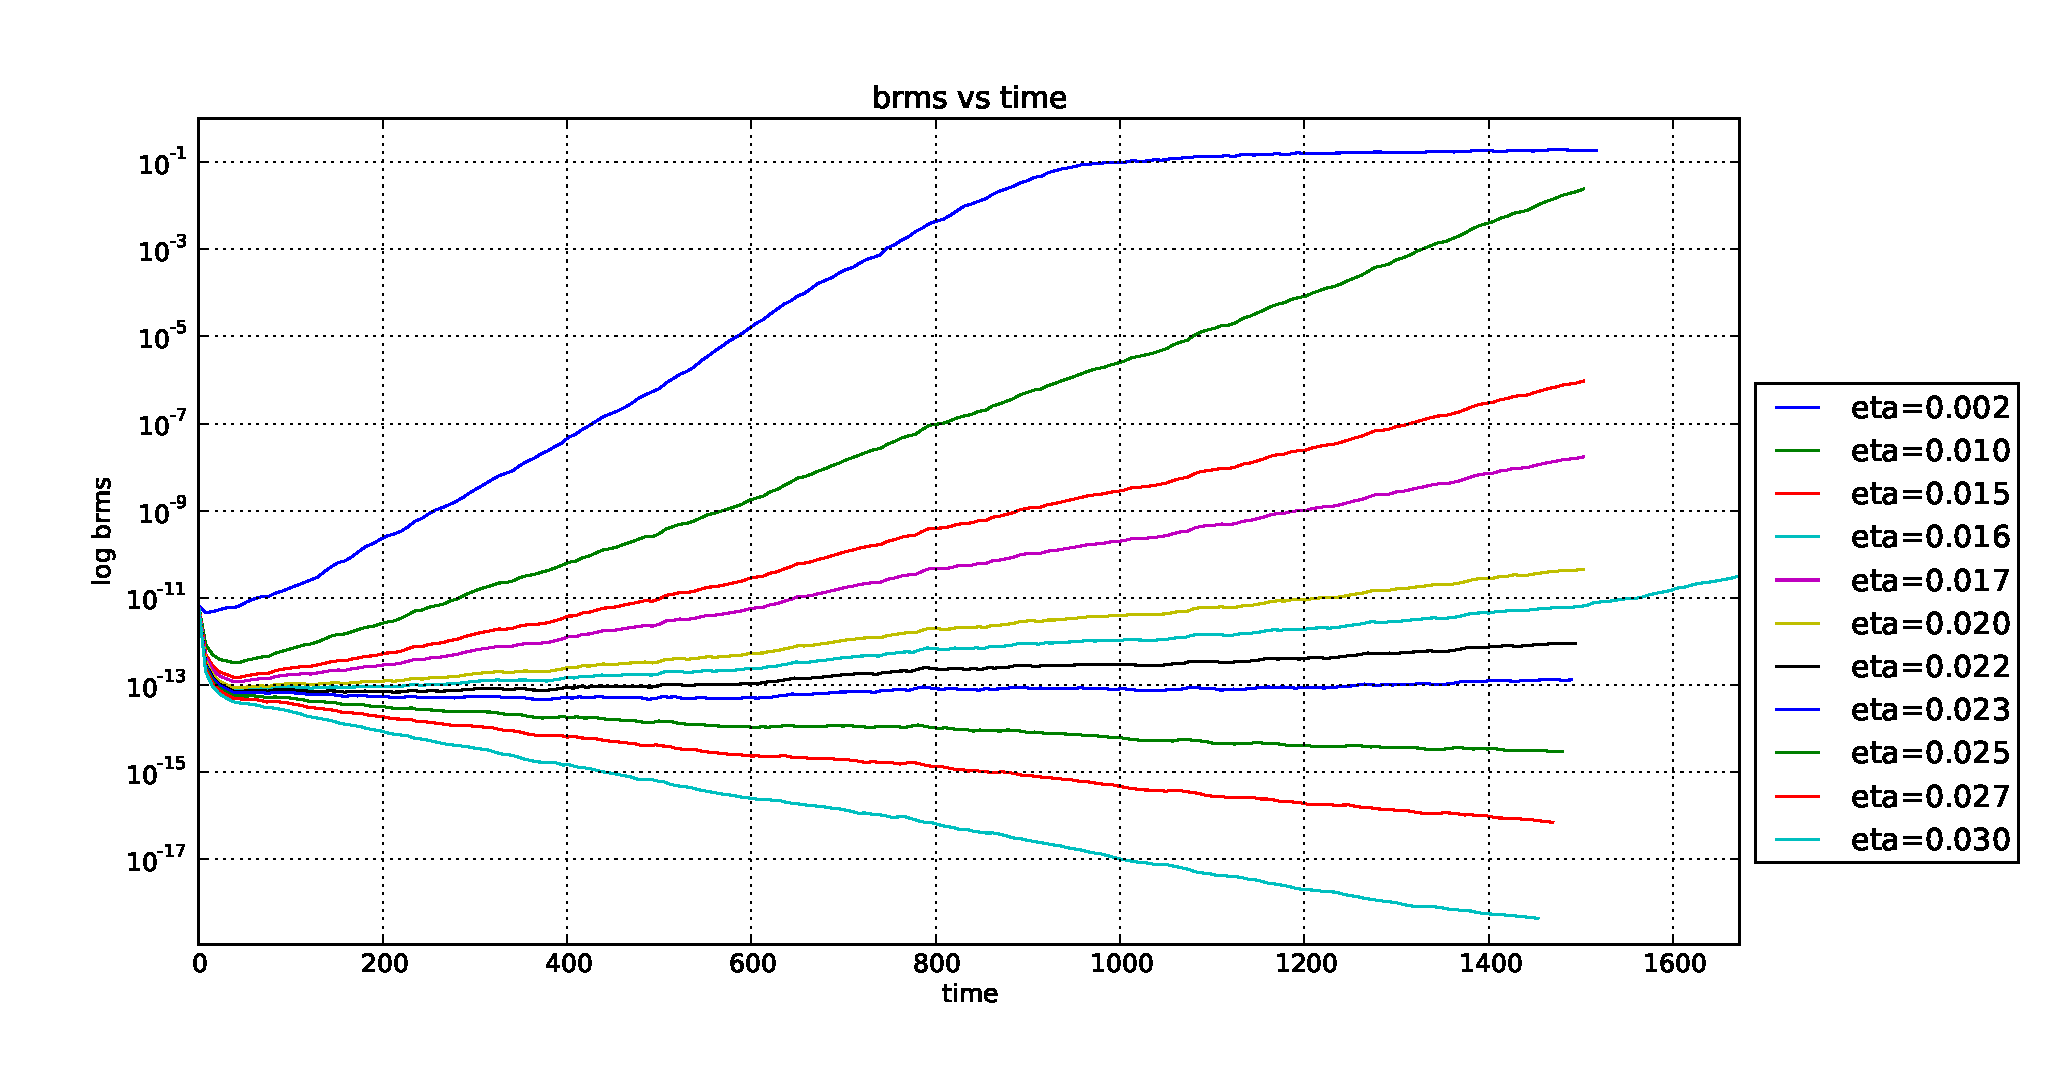
\includegraphics[width=0.8\textwidth]{brms_vs_time.eps}
\caption{log(brms) vs time for different values of  magnetic diffusivity.}
\label{fig:brmst}
 \end{figure}


I tried to find out the critical value for the magnetic diffusivity computing the first derivative of these  curves, restricted to the linear range $100 < t < 900$, and calculating the mean of each derivative. Both quantities are represented in figure \ref{fig:crit_eta}.
\begin{figure}[h]
\centering
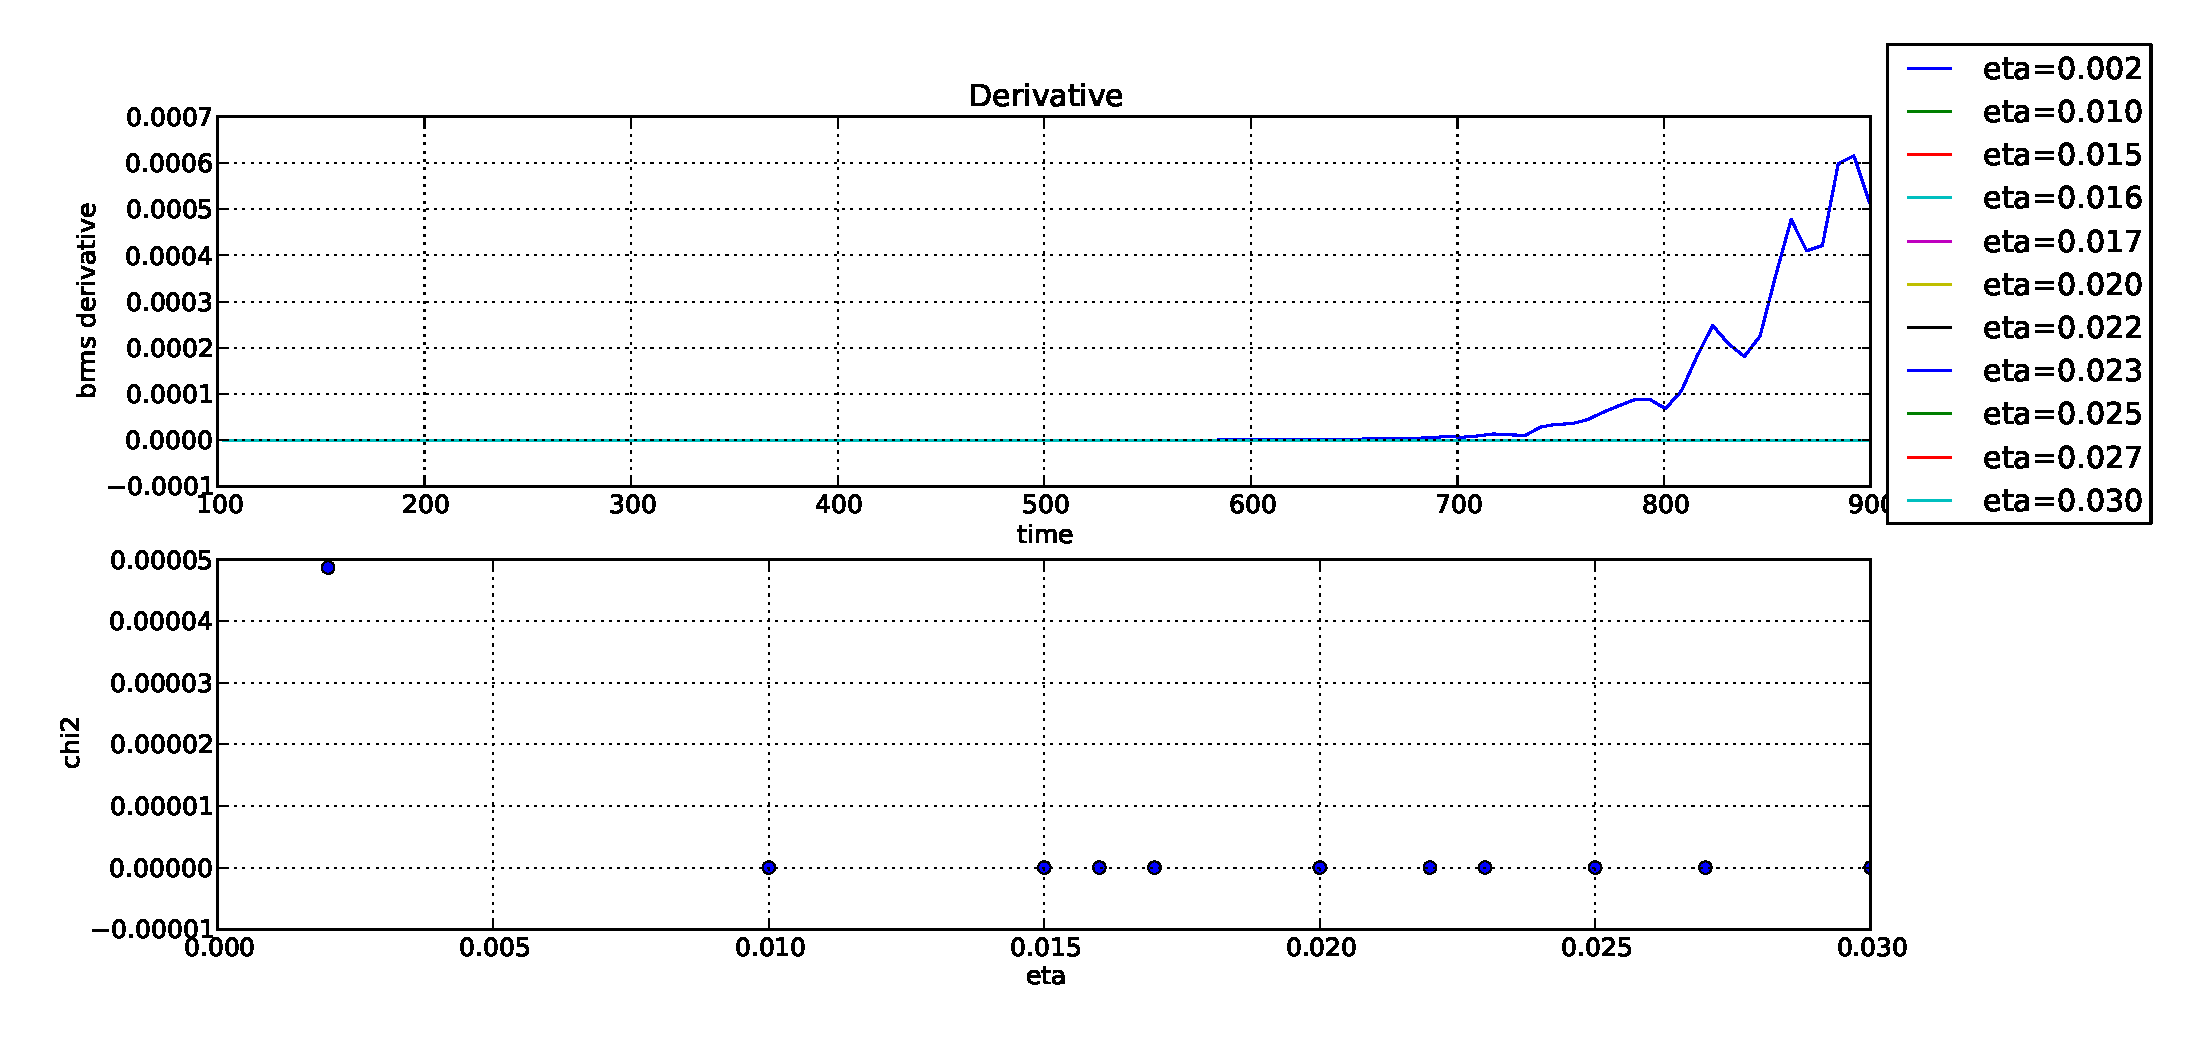
\includegraphics[width=0.8\textwidth]{critical_eta.eps}
\caption{brms derivative vs time and derivative mean for different values of the magnetic diffusivity.}
\label{fig:crit_eta}
 \end{figure}

The mean derivative of the field decreases very quickly to small values:
\begin{center}
\begin{tabular}{ll}
$\eta$ & mean(derivative)\\\hline
2e-3 & 4.87e-05\\
10e-3 & 6.89e-10\\
15e-3 & 1.48e-12\\
16e-3 & 1.04e-15\\
17e-3 & 1.33e-13\\
20e-3 & 3.63e-15\\
22e-3 & 2.63e-16\\
23e-3 & 2.52e-17\\
25e-3 & -5.09e-17\\
27e-3 & -4.54e-17\\
30e-3 & -3.07e-17\\
\end{tabular}
\end{center}

Using these results, I set the critical value for the magnetic diffusivity in $\eta = 22e-3$.

\subsection{Magnetic Reynolds number}
The magnetic Reynolds number is defined as:
\begin{equation}
 Re_M = \frac{u_{rms}}{\eta \kappa_f}
\end{equation}
In this problem I have fixed $\kappa_f = 3$, I found the critical value for the magnetic diffusivity  $\eta = 22e-3$ and the mean value for $u_{rms}$ is $\bar{u_{rms}} = 0.14$, so the corresponding magnetic Reynolds number is $Re_M = 2.15$.

The magnetic Reynolds number is the ratio between convection and diffusion. When $Re_M \gg 1$, convection dominates, whereas for $Re_M \approx 1$, or less, diffusion becomes important. So, in this exercise, diffusion is about to become important.

In fact, the next table shows that $Re_M$ decreases as $\eta$ increases:
\begin{center}
\begin{tabular}{ll}
$\eta$ & $Re_M$\\\hline
2e-3 & 22.39\\
10e-3 & 4.73\\
15e-3 & 3.16\\
16e-3 & 2.97\\
17e-3 & 2.78\\
20e-3 & 2.37\\
22e-3 & 2.15\\
23e-3 & 2.06\\
25e-3 & 1.89\\
27e-3 & 1.75\\
30e-3 & 1.58\\
\end{tabular}
\end{center}

\subsection{Growth rate of the magnetic field}

In order to determine the growth rate of the magnetic field for a value of the magnetic diffusivity, I plotted the logarithm of $brms$ versus time and I did a fit on the sloped part of the curves, as shown in the figures \ref{fig:growth2} and \ref{fig:growth10}.

\begin{figure}[h]
\begin{minipage}[t]{.45\textwidth}
\centering
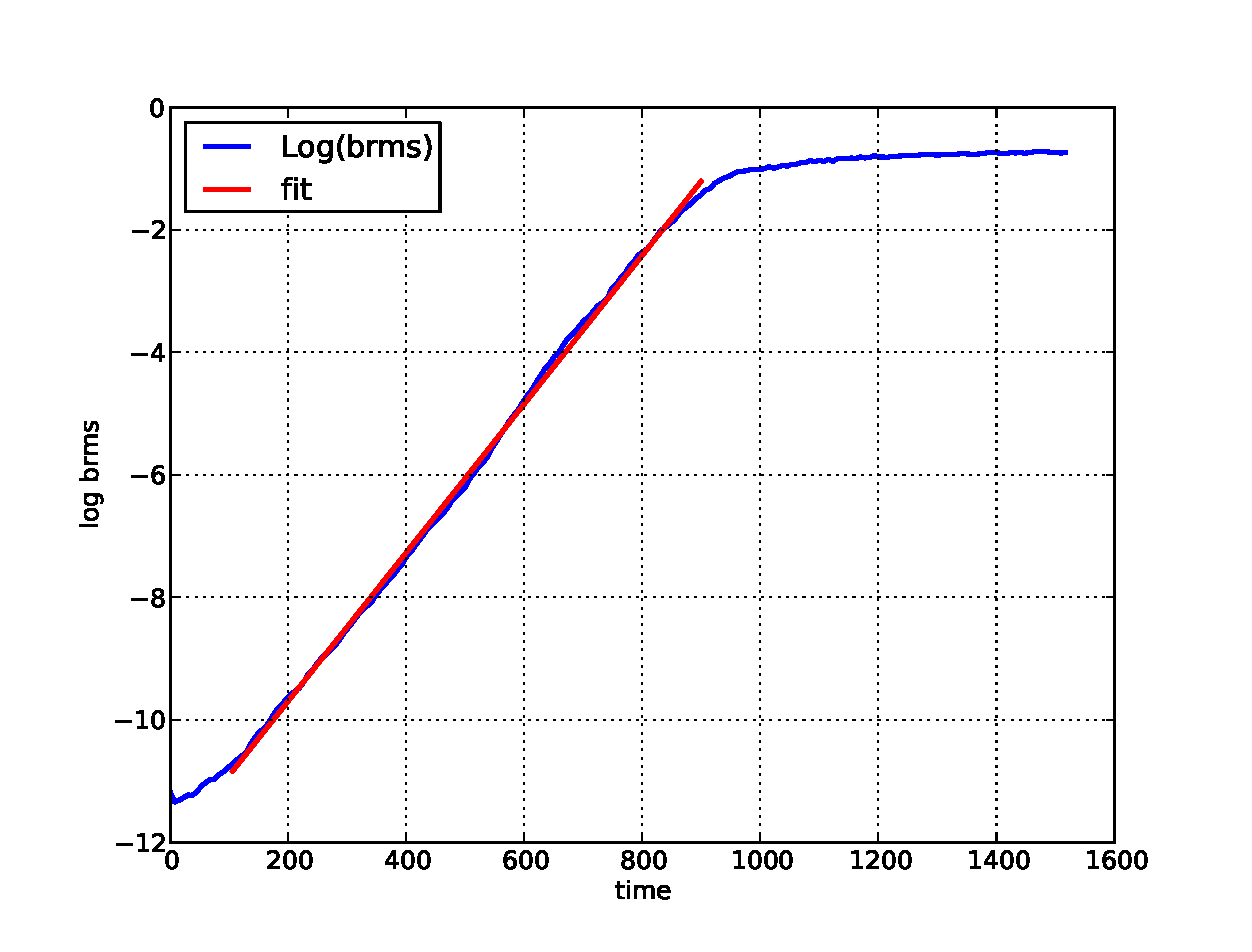
\includegraphics[width=\textwidth]{growth2e-3.eps}
\caption{Growth rate of the magnetic field for a value of the magnetic diffusivity  $\eta = 2e-3$.}
\label{fig:growth2}
\end{minipage}
\hspace{0.5cm}
\begin{minipage}[t]{.45\textwidth}
\centering
 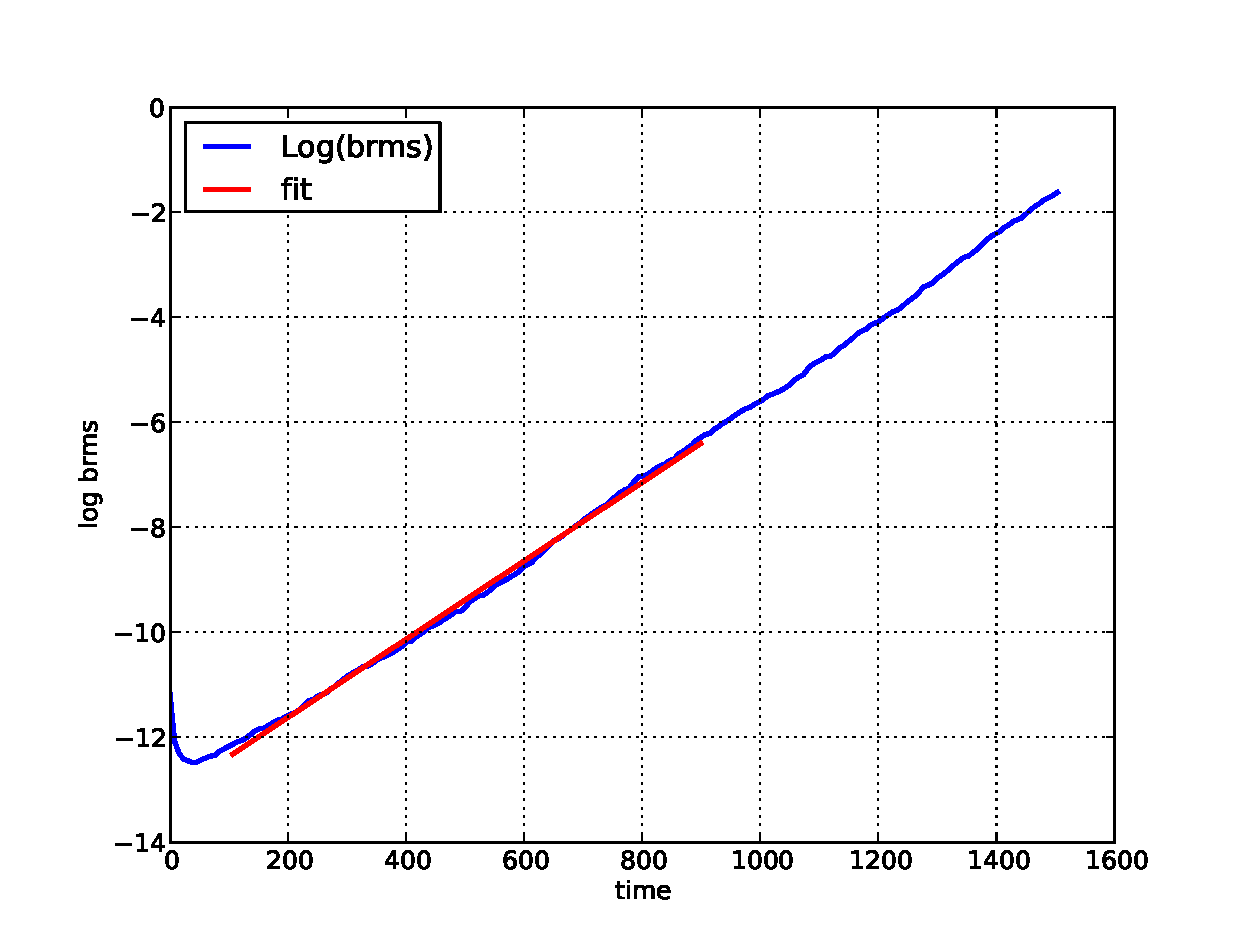
\includegraphics[width=\textwidth]{growth10e-3.eps}
\caption{Growth rate of the magnetic field for a value of the magnetic diffusivity  $\eta = 10e-3$.}
\label{fig:growth10}
\end{minipage}
 \end{figure}
%y=ax+b
The parameter $a$ in a linear regression fit ($y=ax+b$) is a measure of the growth rate of the magnetic field. The growth depends on the value of the magnetic diffusivity, and it decreases as the magnetic diffusivity increases.
\begin{center}
\begin{tabular}{lll}
$\eta$ & a & b\\\hline
2e-3 & 0.0121 & -12.12\\
10e-3 & 0.0075 & -13.11
\end{tabular}
\end{center}

\subsection{Structure of the magnetic field.}

Figure \ref{fig:averages} shows the evolution of three different magnetic field averages: the xy average bmz, the yz average bmx and the zx average bmy. 
From the figure one can see that the $zx$ average dominates in the end.
\begin{figure}[h]
\centering
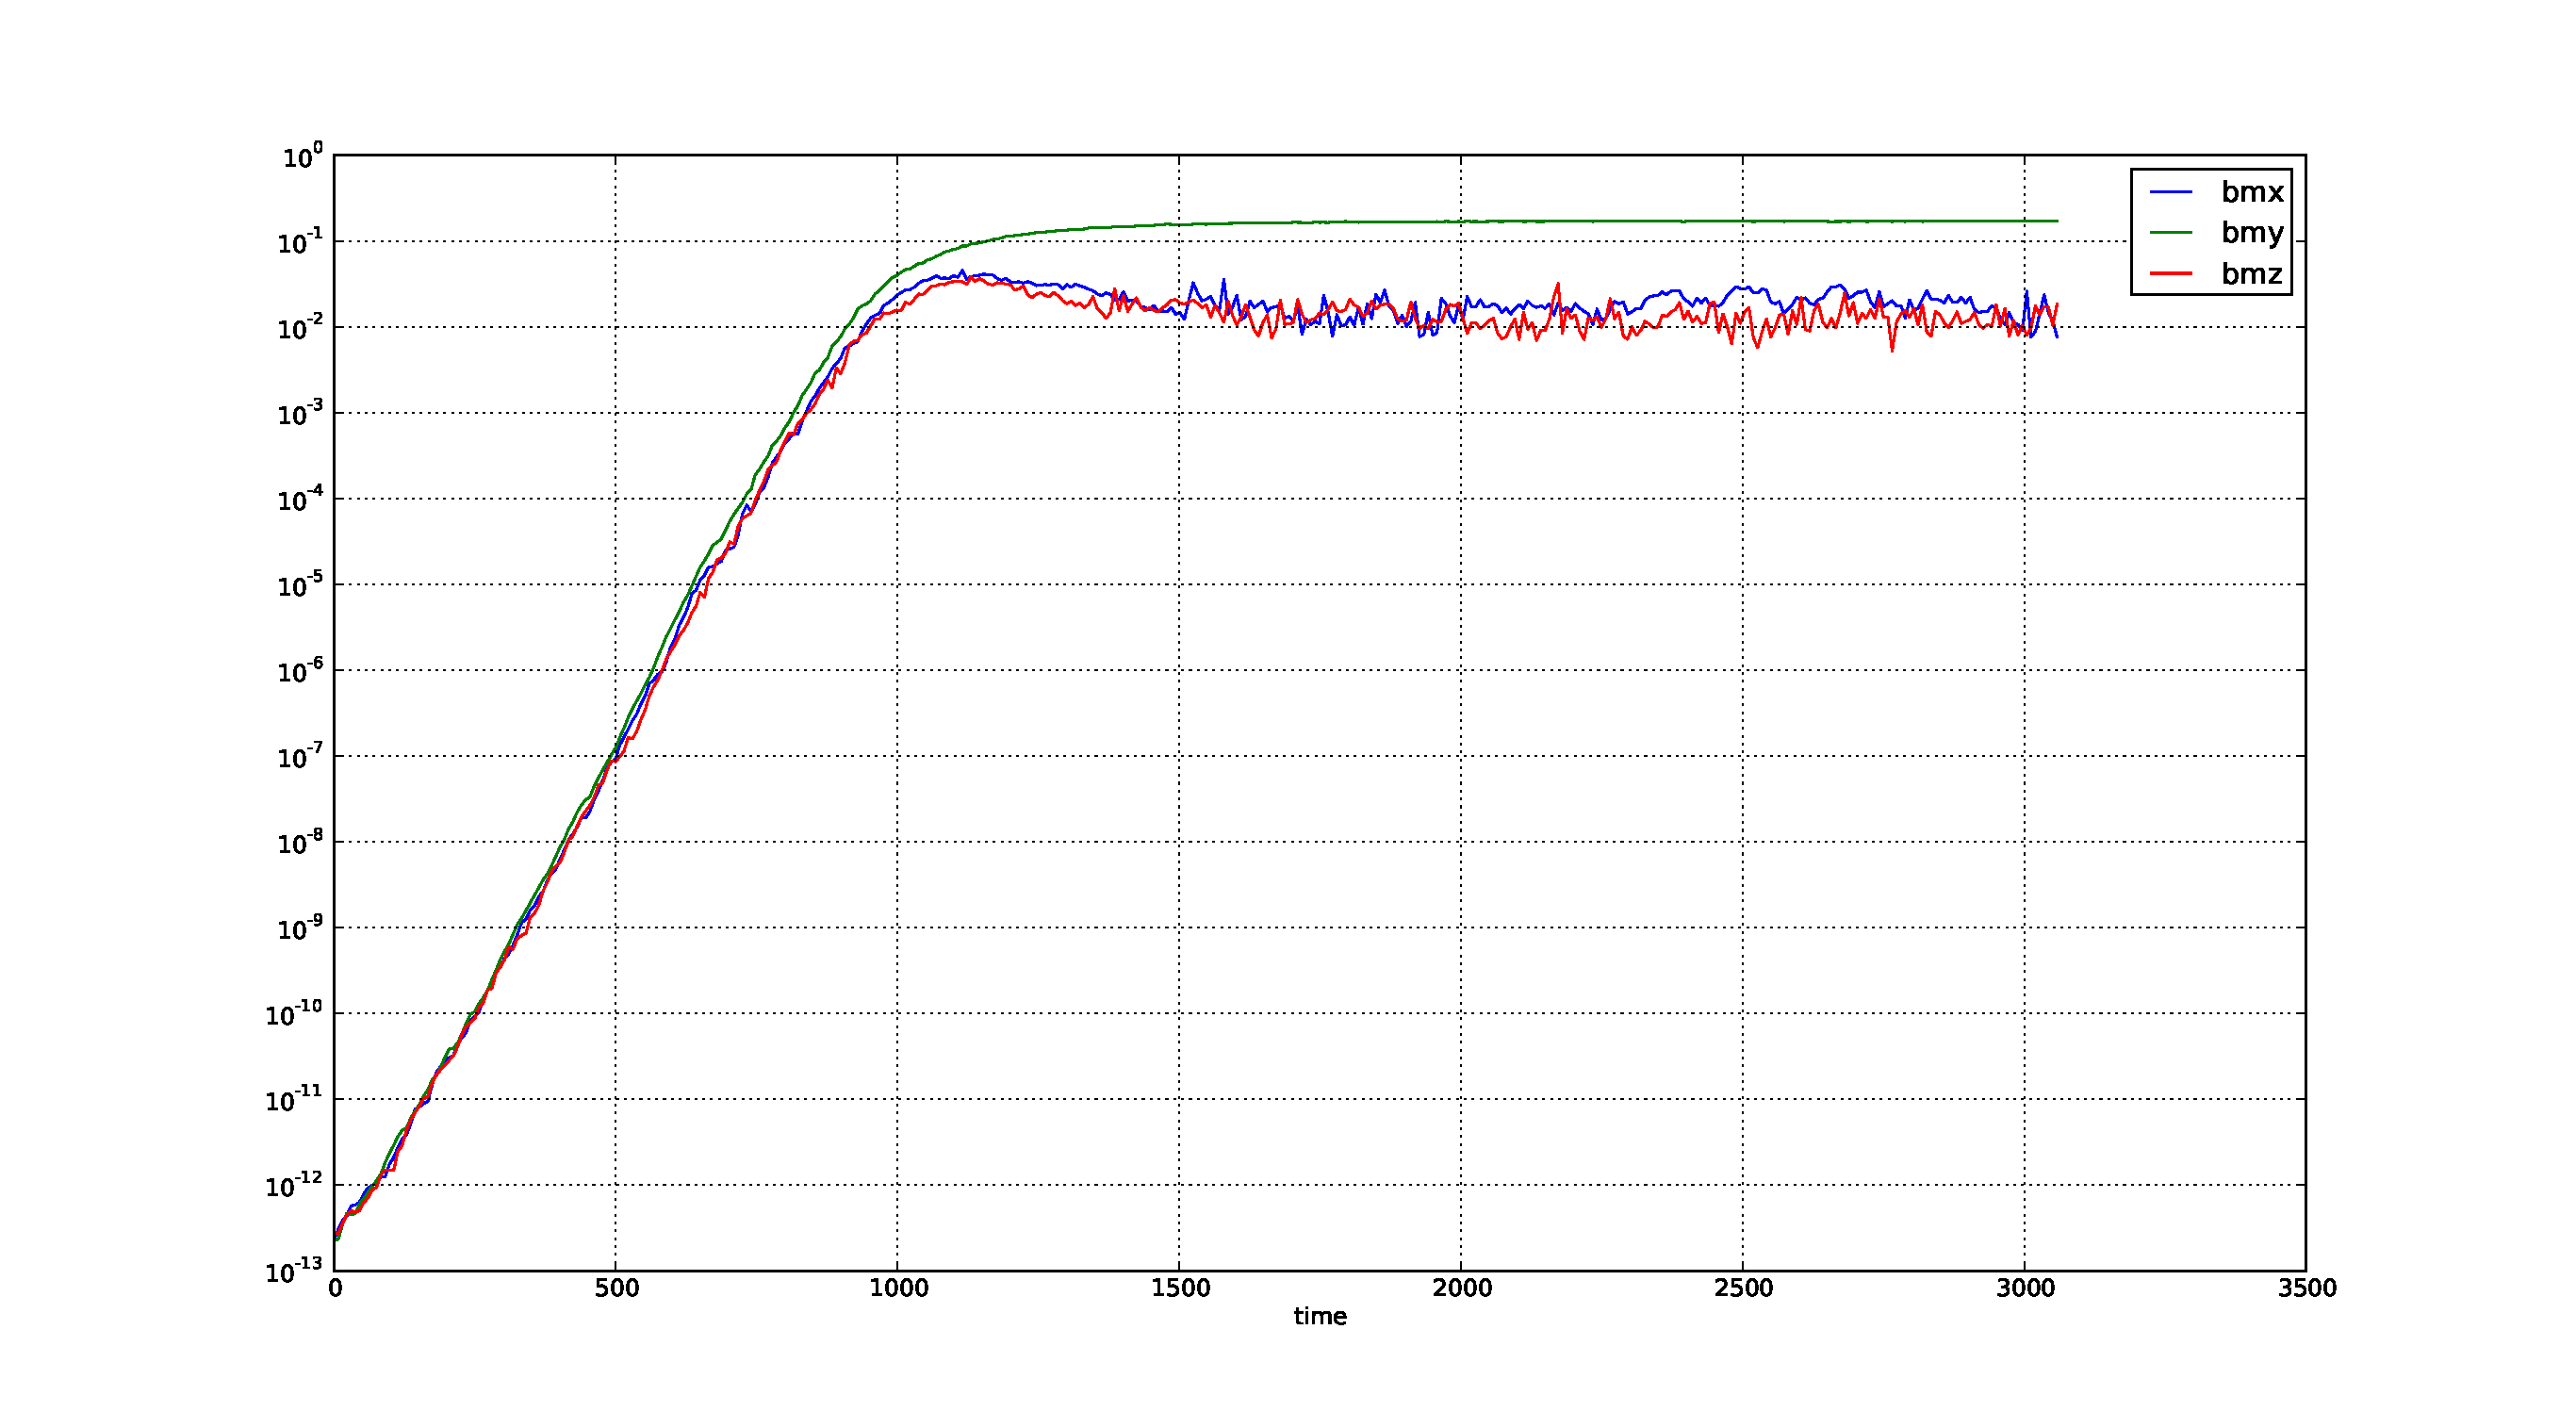
\includegraphics[width=0.8\textwidth]{campos3.eps}
\caption{Averages of three different magnetic fields.}
\label{fig:averages}
 \end{figure}

\subsection{Fitting $B_{zx}$}
Fitting the strongest of the three field averages $<\bar{B^2}>$ to the expression:
\begin{equation}
 F(t;B_0,t_s)=B_0^2[1-\exp^{-2\eta\kappa_1^2(t-t_s)}]
\label{eq:fitB}
\end{equation}
The strongest of the three field averages is the zx average represented in the figure \ref{fig:bmy_fit} with different values of the expression \ref{eq:fitB}.
\begin{figure}[h]
\centering
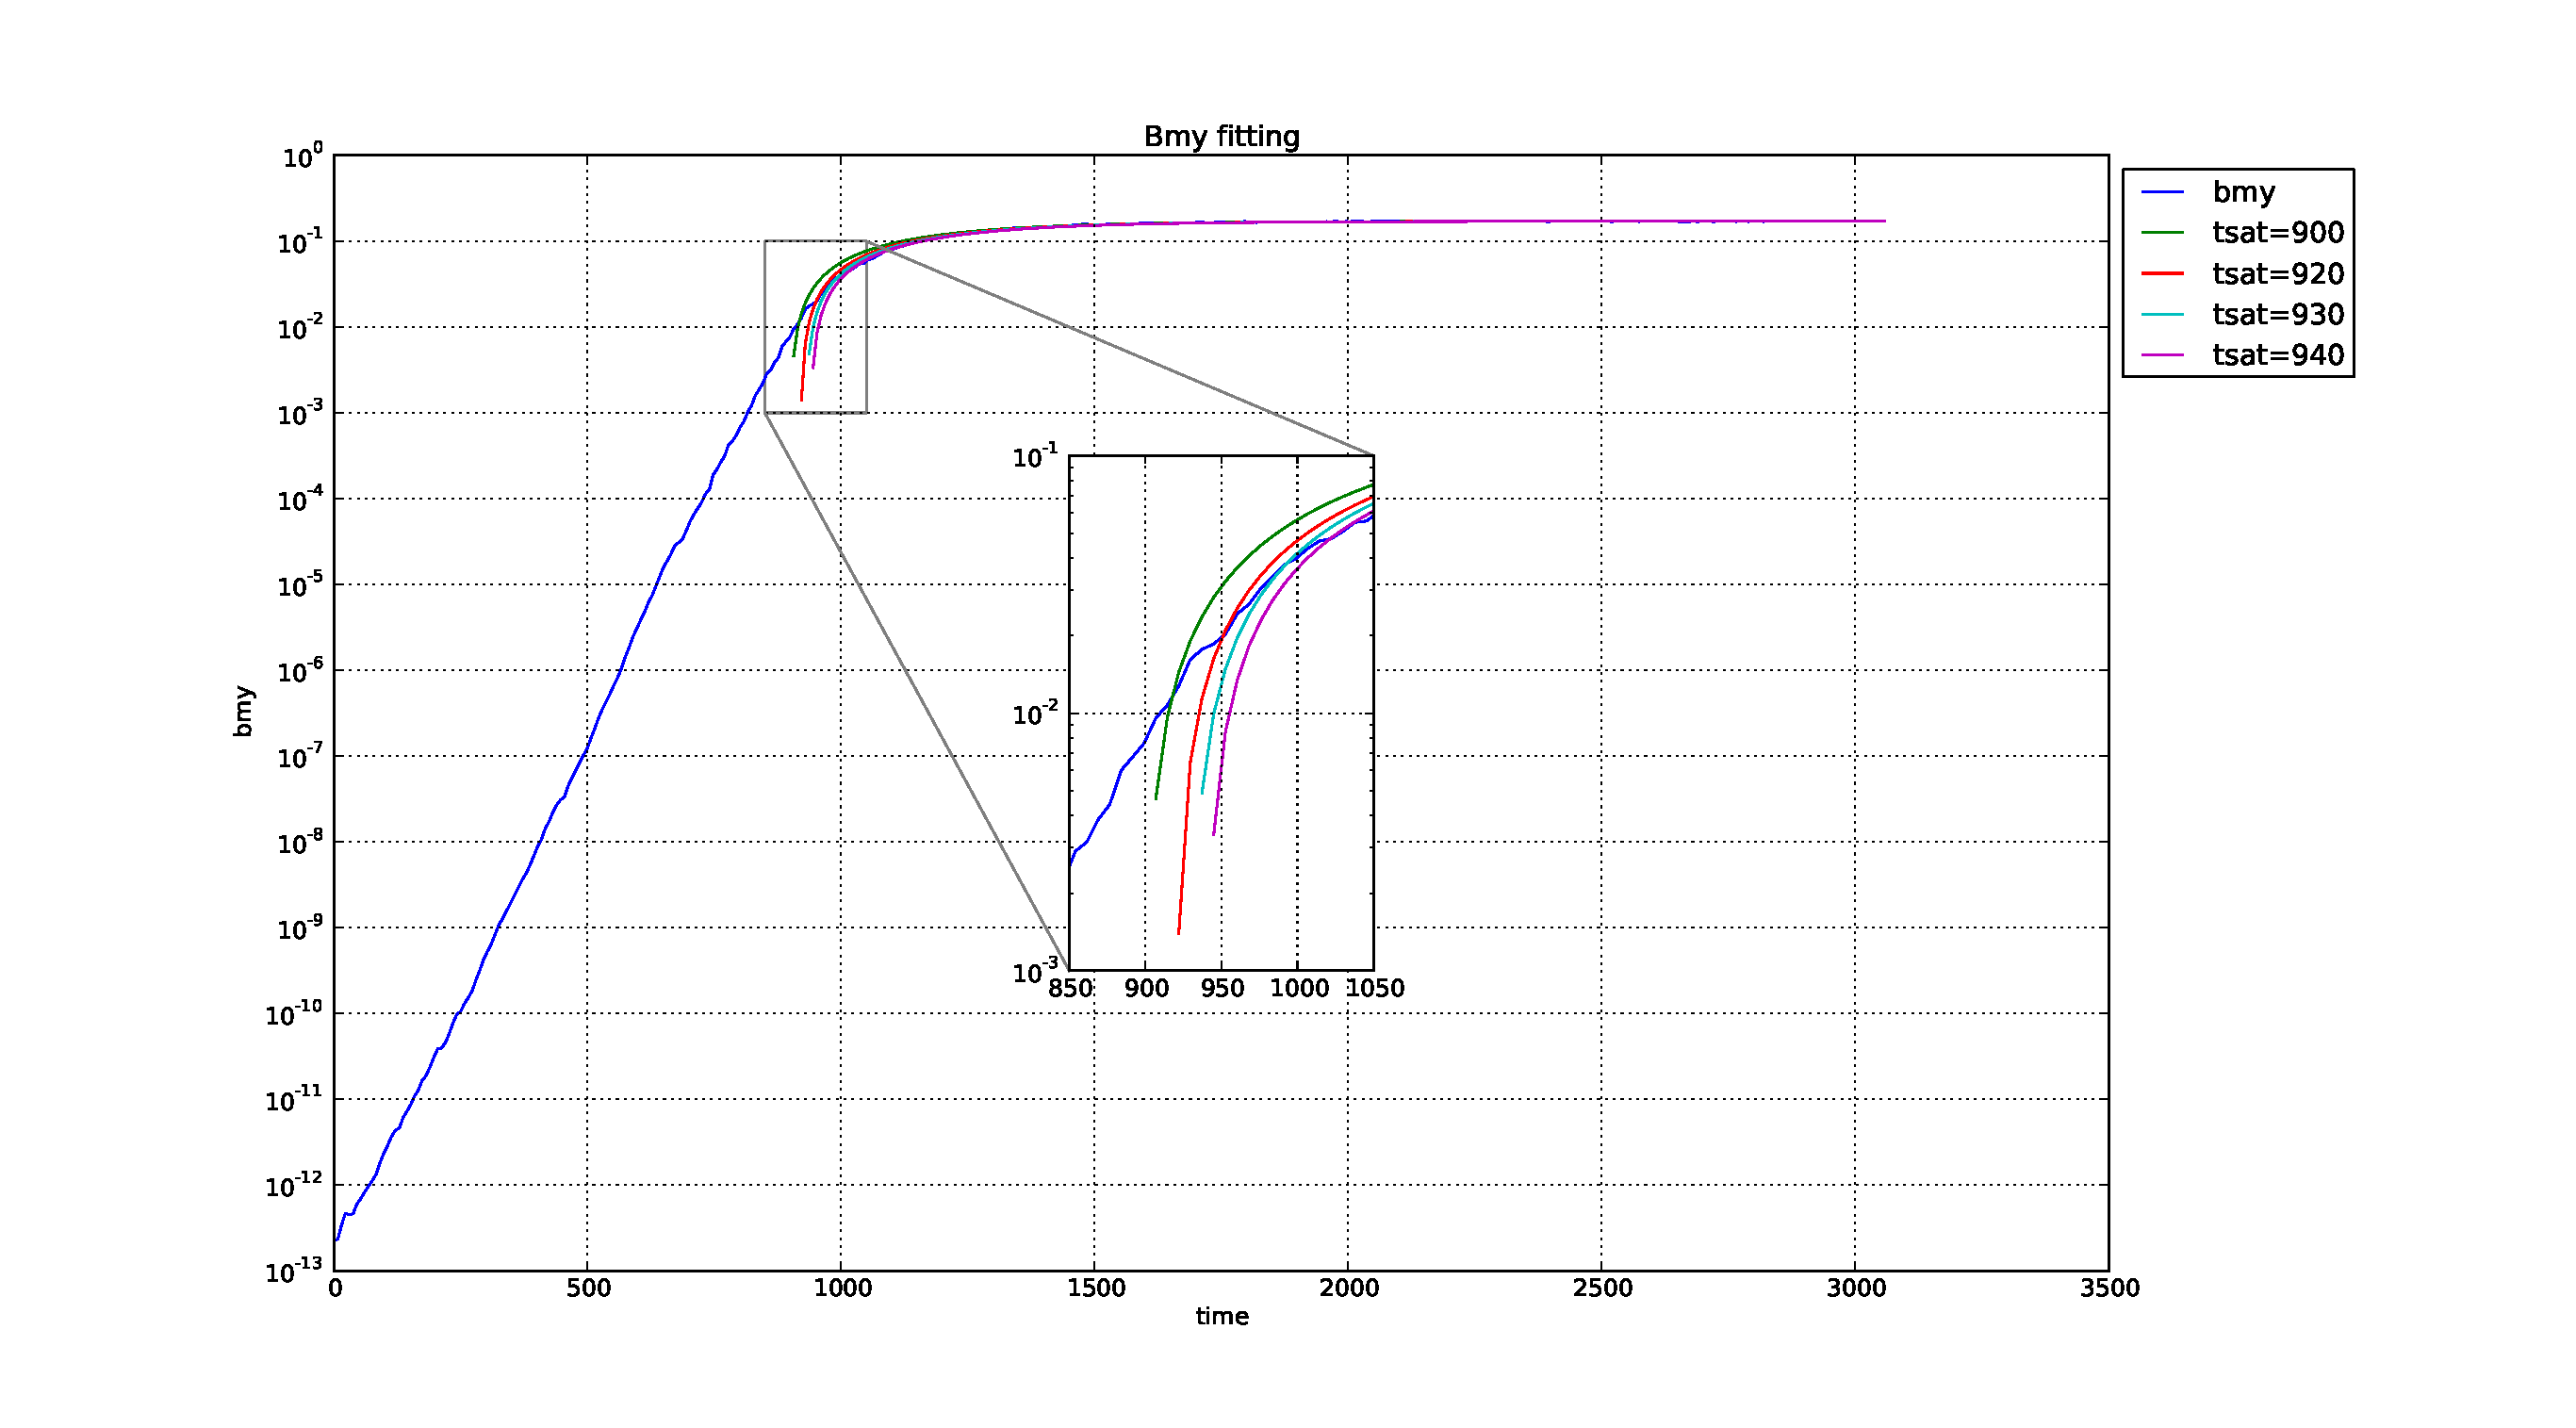
\includegraphics[width=0.8\textwidth]{bmy_fit.eps}
\caption{Bmy Fitting: $B_0=0.1712$ and $t_s = 930$.}
\label{fig:bmy_fit}
 \end{figure}
A rough fit for the field average takes the values $B_0=0.1712$ and $t_s = 930$.
$B_0$ is the saturation field value and $t_s$ is the best fit curve just before saturation.

In order to do a best mathematical fit a likelihood method could be used: 
\begin{itemize}
 \item Compute the function:
\begin{equation}
 G(t_s) = \sum_{t=a}^b (<\bar{B}^2_{(t)}>-F(t;B_0,t_s))
\end{equation}
\item Find the $t_s$ value which minimizes this function, using, for example, the false position method.

\end{itemize}



\end{document}
